%*----------- SLIDE -------------------------------------------------------------
\begin{frame}[t]{Ciclo Ingênuo}
    
    \begin{columns}
        \column{.01\textwidth}
        \column{.5\textwidth}
            \centering
            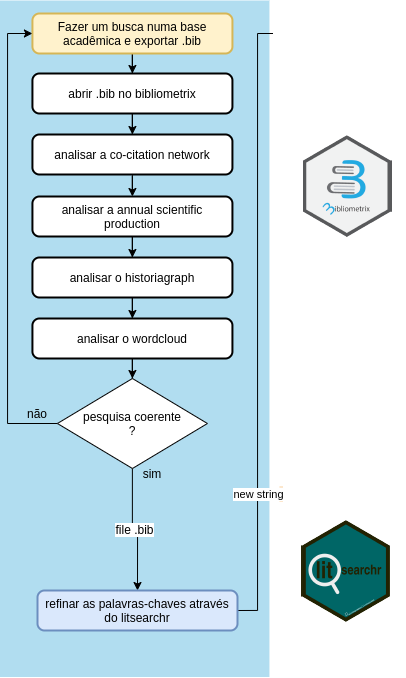
\includegraphics[width=.55\textwidth, trim= 0 0 0 0, clip]{ciclo1.png}
        \column{.6\textwidth}
            \centering
            Fazer uma busca numa base acadêmica e exportar no formato \emph{.bib}\\

            \vspace*{0.2cm}
            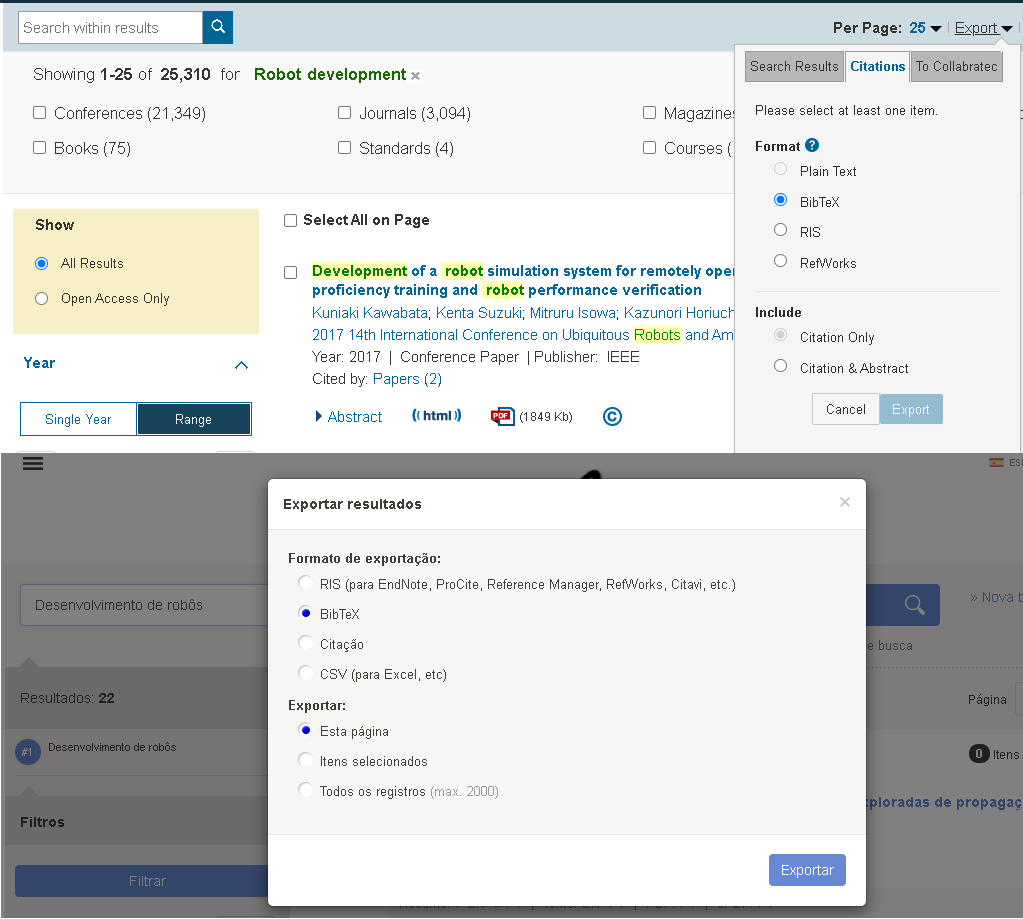
\includegraphics[width=.55\textwidth, trim= 0 0 0 0, clip]{bases.png}
    \end{columns}

%*----------- notes
    \note[item]{Notes can help you to remember important information. Turn on the notes option.}
\end{frame}
%-
%*----------- SLIDE -------------------------------------------------------------
\begin{frame}[t]{Ciclo Ingênuo}
    
    % \begin{columns}
    %     \column{.01\textwidth}
    %     \column{.5\textwidth}
    %         \centering
    %         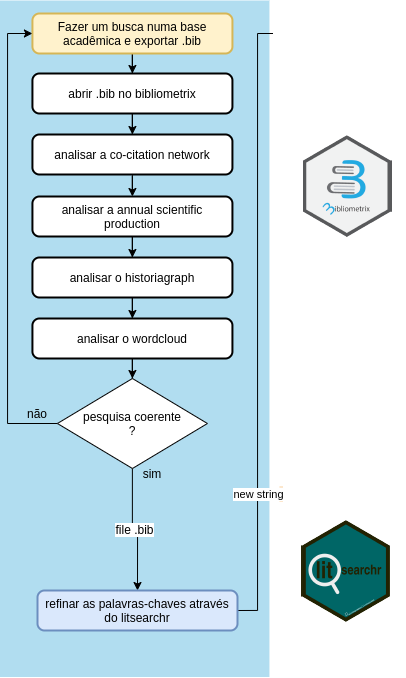
\includegraphics[width=.55\textwidth, trim= 0 0 0 0, clip]{ciclo1.png}
    %     \column{.6\textwidth}
    %         \centering
    %         Fazer uma busca numa base acadêmica e exportar no formato \emph{.bib}\\

    %         \vspace*{0.2cm}
    %         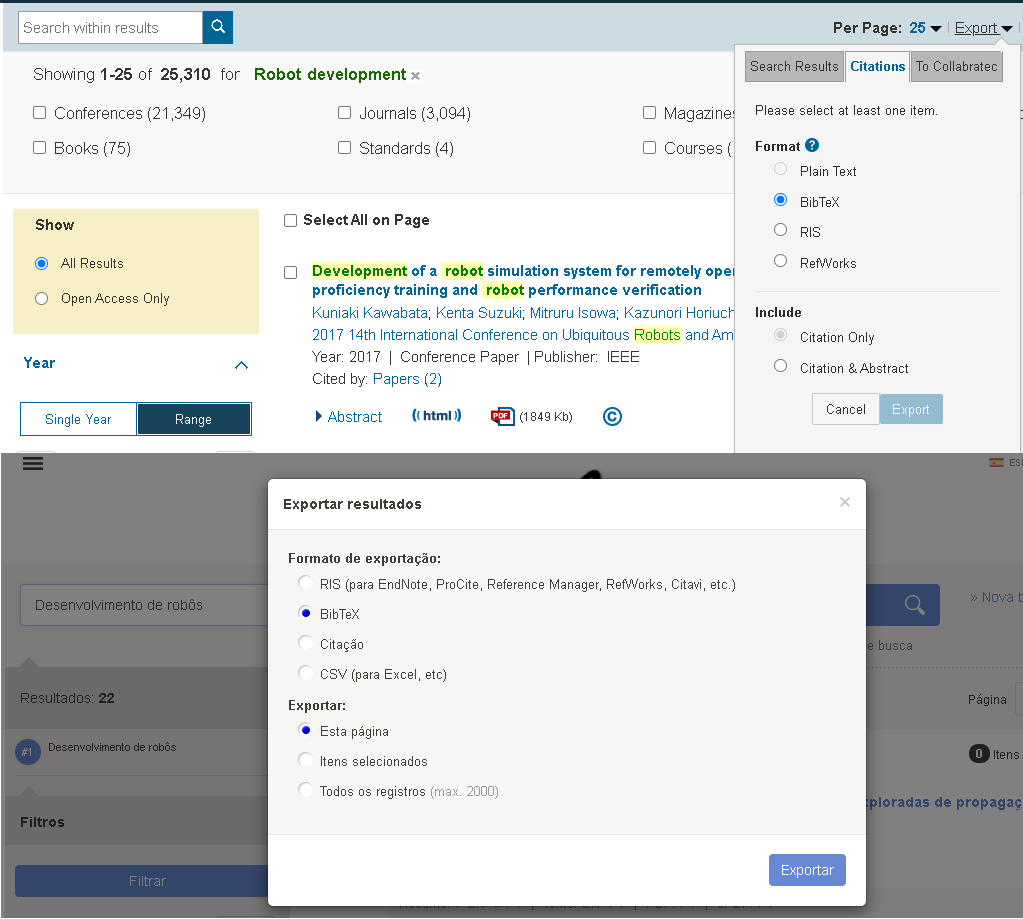
\includegraphics[width=.55\textwidth, trim= 0 0 0 0, clip]{bases.png}
    % \end{columns}
    \begin{tcolorbox}[colback=gcolor!5!white,colframe=gcolor!75!black,title=String]
        (("underwater manipulator" OR "underwater vehicle manipulator system") AND ("underwater robot" OR "underwater vehicle" OR "autonomous underwater") AND ("disturbance observer"))
    \end{tcolorbox}

    \centering
    \centerline{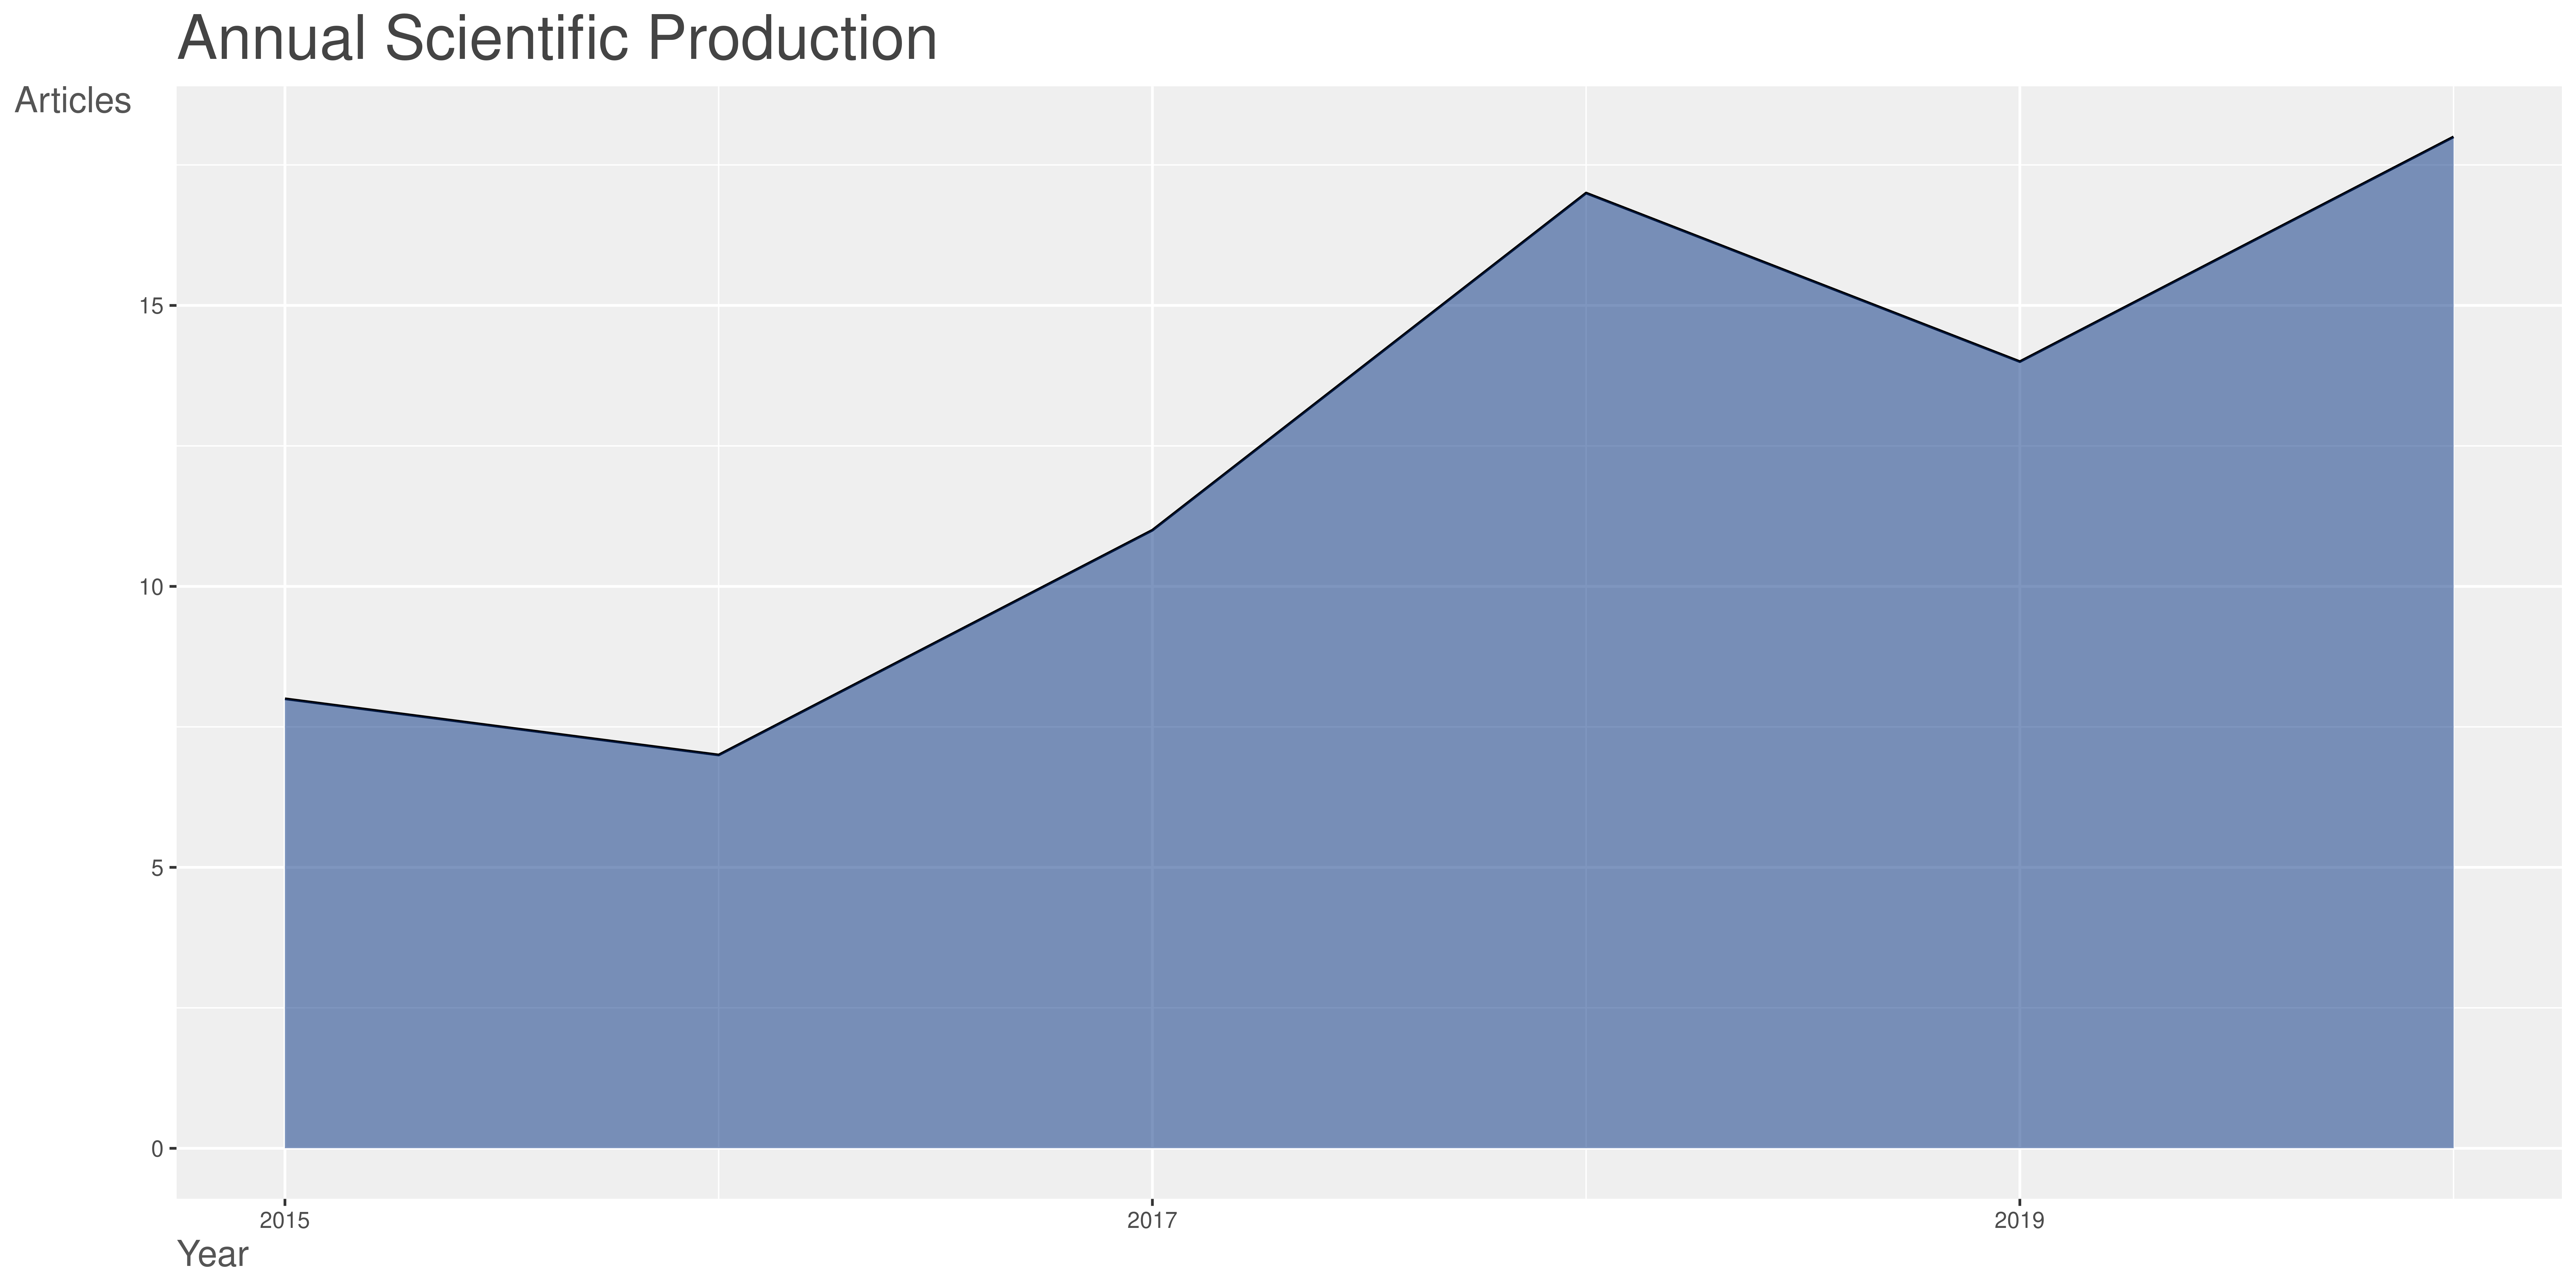
\includegraphics[trim = 0 0 0 0, clip, width=0.5\textwidth]{AnnualScientificProduction-2021-04-28.png}}

%*----------- notes
    \note[item]{Notes can help you to remember important information. Turn on the notes option.}
\end{frame}
%-
%*----------- SLIDE -------------------------------------------------------------
\begin{frame}[t]{Ciclo Ingênuo}
    
    % \begin{columns}
    %     \column{.01\textwidth}
    %     \column{.5\textwidth}
    %         \centering
    %         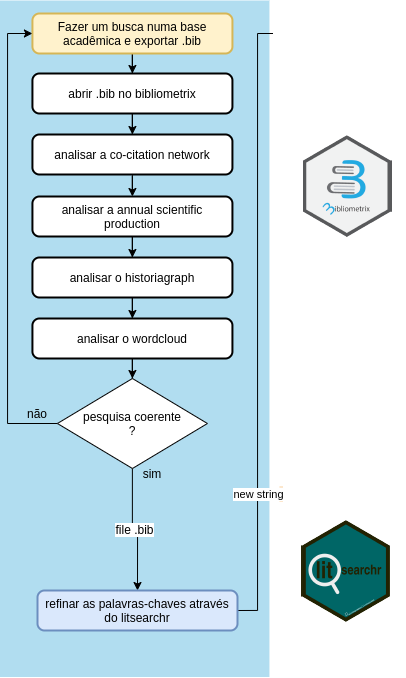
\includegraphics[width=.55\textwidth, trim= 0 0 0 0, clip]{ciclo1.png}
    %     \column{.6\textwidth}
    %         \centering
    %         Fazer uma busca numa base acadêmica e exportar no formato \emph{.bib}\\

    %         \vspace*{0.2cm}
    %         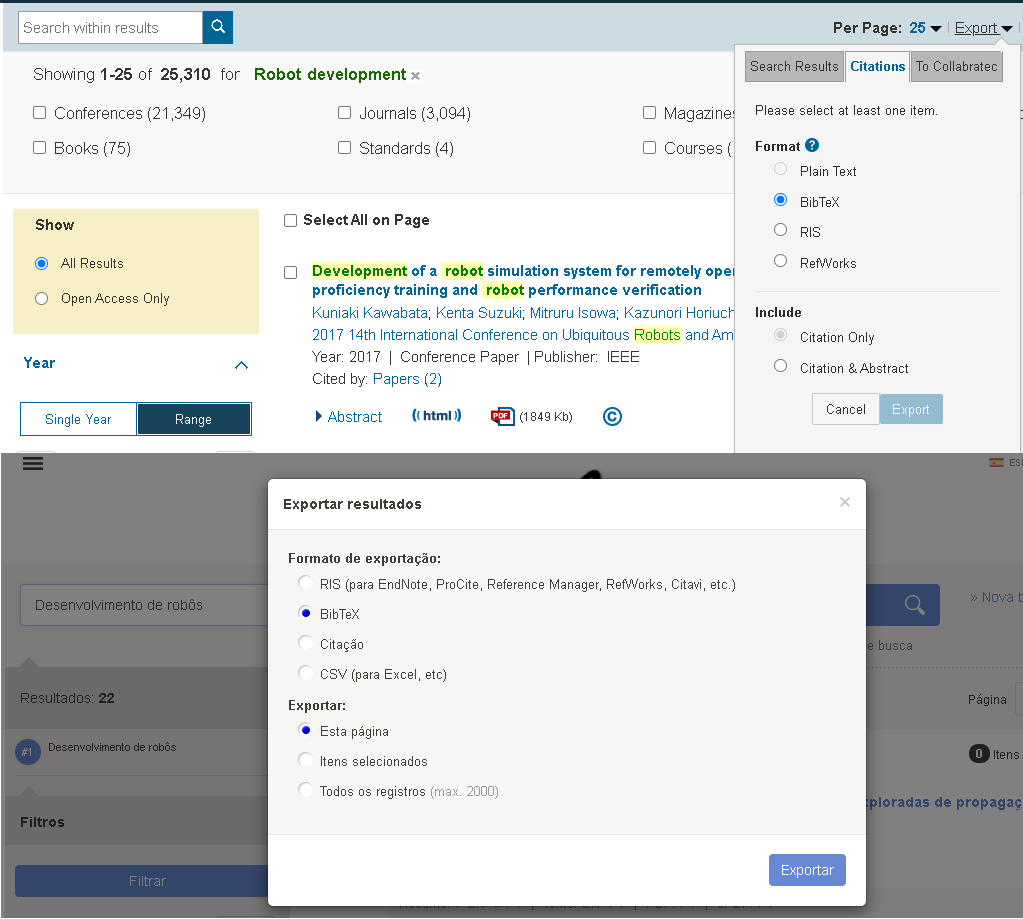
\includegraphics[width=.55\textwidth, trim= 0 0 0 0, clip]{bases.png}
    % \end{columns}
    \centering
    \centerline{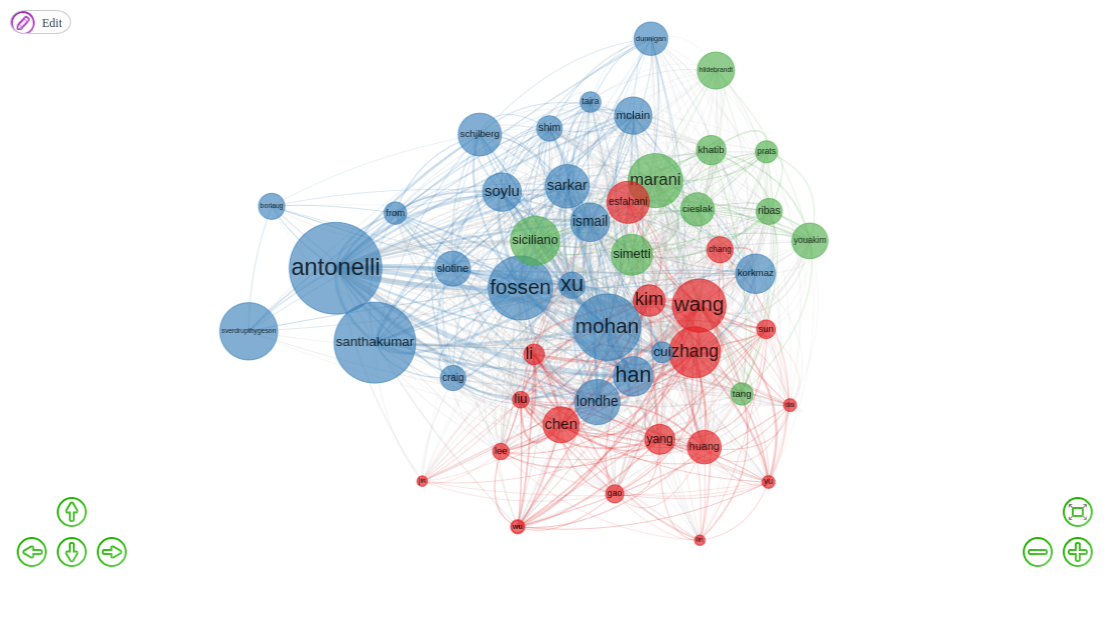
\includegraphics[trim = 0 0 0 0, clip, width=.9\textwidth]{network (3).png}}

%*----------- notes
    \note[item]{Notes can help you to remember important information. Turn on the notes option.}
\end{frame}
%-
%*----------- SLIDE -------------------------------------------------------------
\begin{frame}[t]{uma nova string}
    
    \centering
    \centerline{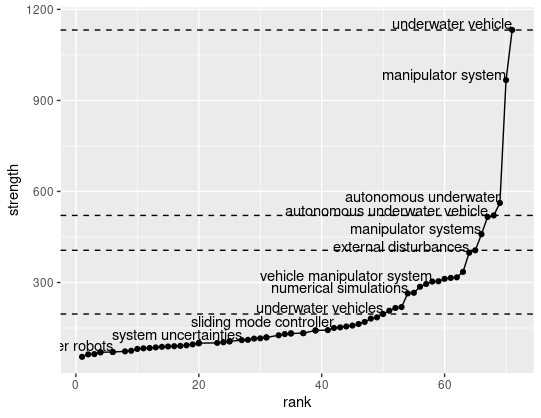
\includegraphics[trim = 0 0 0 0, clip, width=0.35\textwidth]{Rplot03.png}}

    \centering
    \centerline{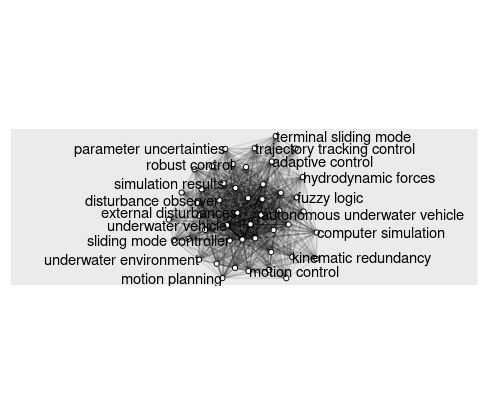
\includegraphics[trim = 0 70 0 80, clip, width=0.5\textwidth]{Rplot04.png}}


%*----------- notes
    \note[item]{Notes can help you to remember important information. Turn on the notes option.}
\end{frame}
%-
%*----------- SLIDE -------------------------------------------------------------
\begin{frame}[c]{uma nova string}
    
    \begin{tcolorbox}[colback=gcolor!5!white,colframe=gcolor!75!black,title=String Refinada]
        (("manipulator system" OR "underwater manipulator" OR "vehicle manipulator system" OR "underwater vehicle manipulator system") AND ("underwater manipulator" OR "underwater robot" OR "underwater vehicle" OR "autonomous underwater") AND ("disturbance observer" OR "external disturbances" OR "motion planning" OR "trajectory tracking" OR "sliding mode control"))
    \end{tcolorbox}

    
%*----------- notes
    \note[item]{Notes can help you to remember important information. Turn on the notes option.}
\end{frame}
%-
%*----------- SLIDE -------------------------------------------------------------
\begin{frame}[t]{Ciclo Otimizado}
    
    \begin{columns}
        \column{.01\textwidth}
        \column{.5\textwidth}
            \centering
            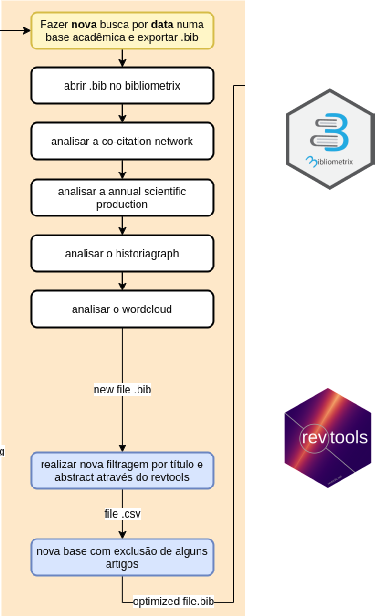
\includegraphics[width=.55\textwidth, trim= 0 0 0 0, clip]{ciclo2.png}
        \column{.6\textwidth}
            \centering
            Testar a nova \emph{string}, e exportar os dados otimizado no formato \emph{.bib}\\

            \vspace*{0.2cm}
            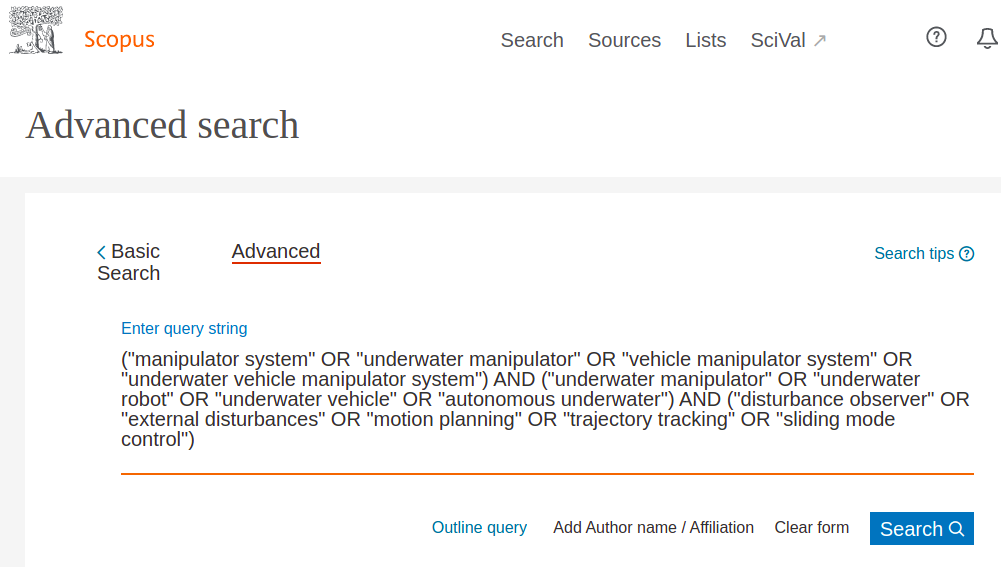
\includegraphics[width=.85\textwidth, trim= 0 0 0 0, clip]{novabusca.png}
    \end{columns}

%*----------- notes
    \note[item]{Notes can help you to remember important information. Turn on the notes option.}
\end{frame}
%-
%*----------- SLIDE -------------------------------------------------------------
\begin{frame}[c]{Ciclo Otimizado}
    
    \begin{columns}
        \column{.01\textwidth}
        \column{.5\textwidth}
            \centering
            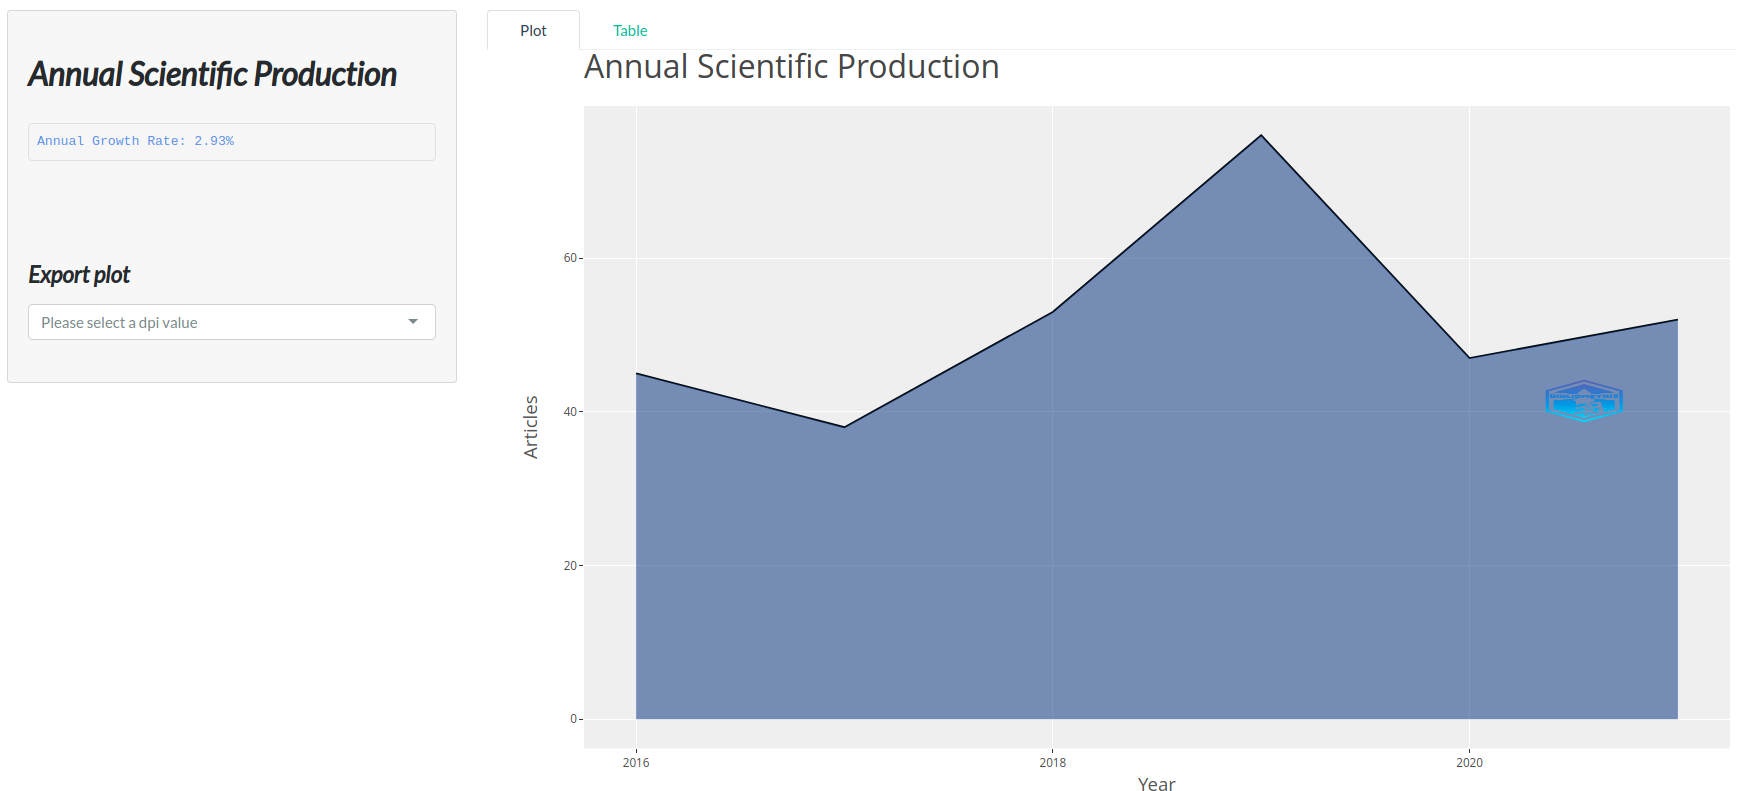
\includegraphics[width=1\textwidth, trim= 500 0 0 0, clip]{turbot1.png}
        \column{.5\textwidth}
            \centering
            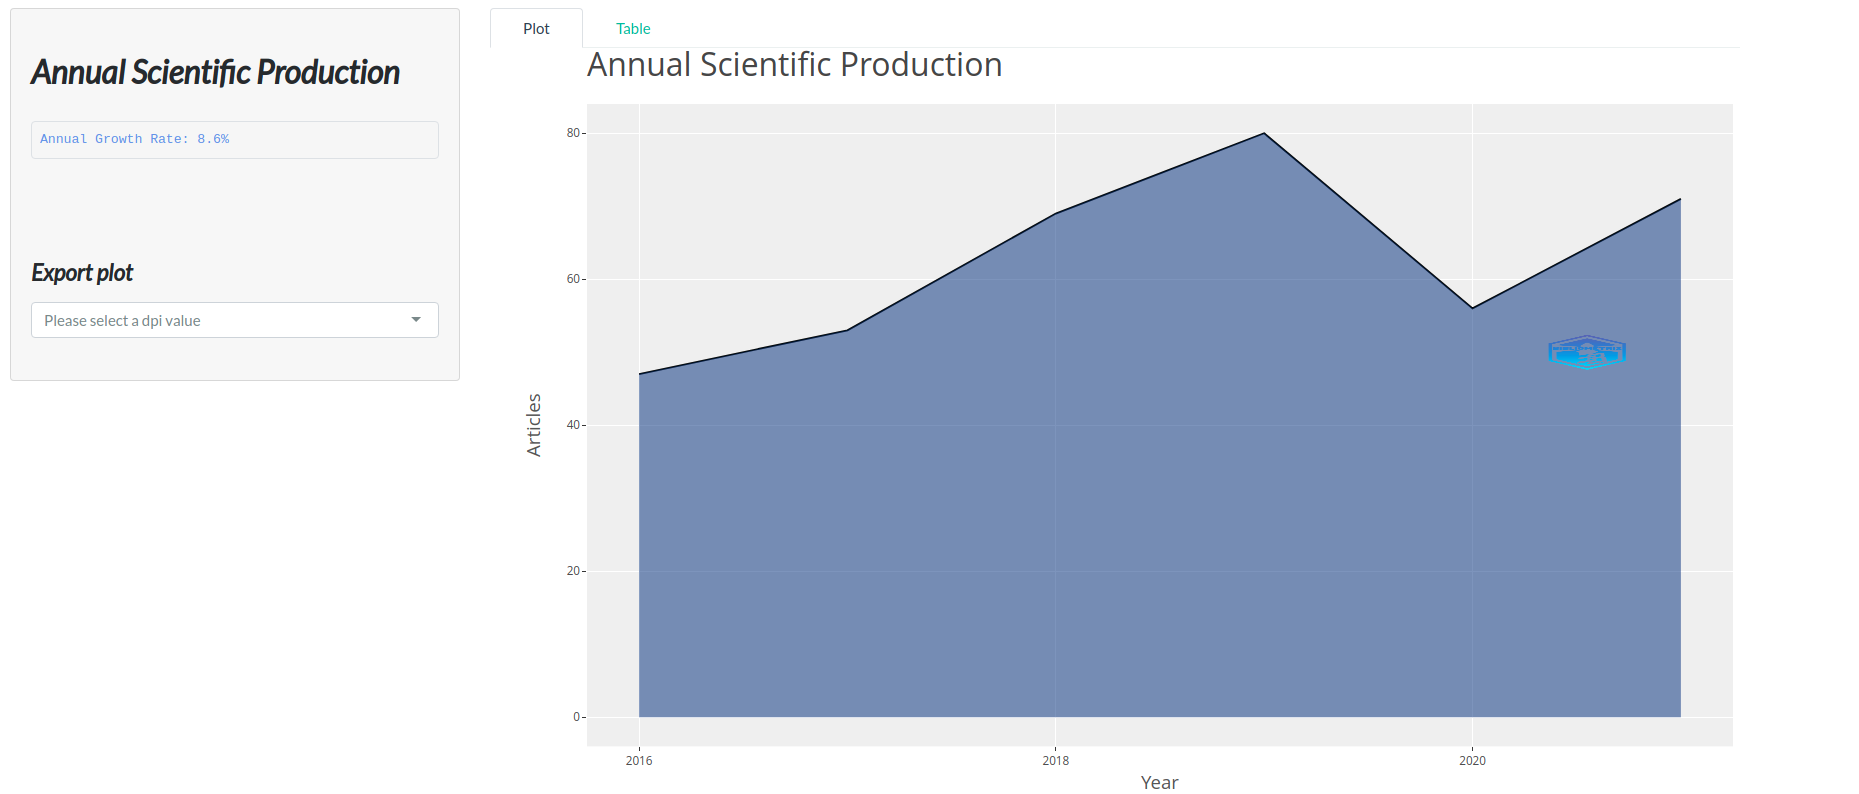
\includegraphics[width=1\textwidth, trim= 500 0 100 0, clip]{turbot2.png}

    \end{columns}

%*----------- notes
    \note[item]{Notes can help you to remember important information. Turn on the notes option.}
\end{frame}
%-
%*----------- SLIDE -------------------------------------------------------------
\begin{frame}[c]{Ciclo Otimizado}
    
    \begin{columns}
        \column{.01\textwidth}
        \column{.5\textwidth}
            \centering
            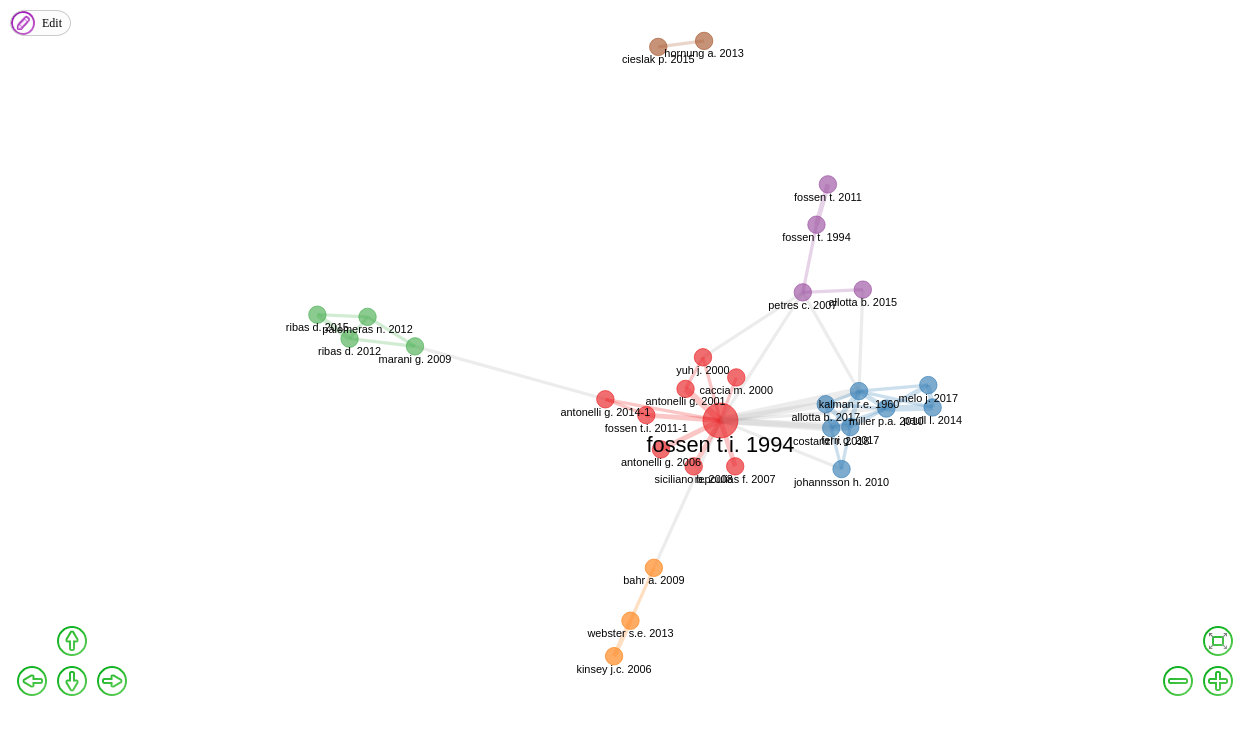
\includegraphics[width=1\textwidth, trim= 200 0 200 0, clip]{turbot3.png}
        \column{.5\textwidth}
            \centering
            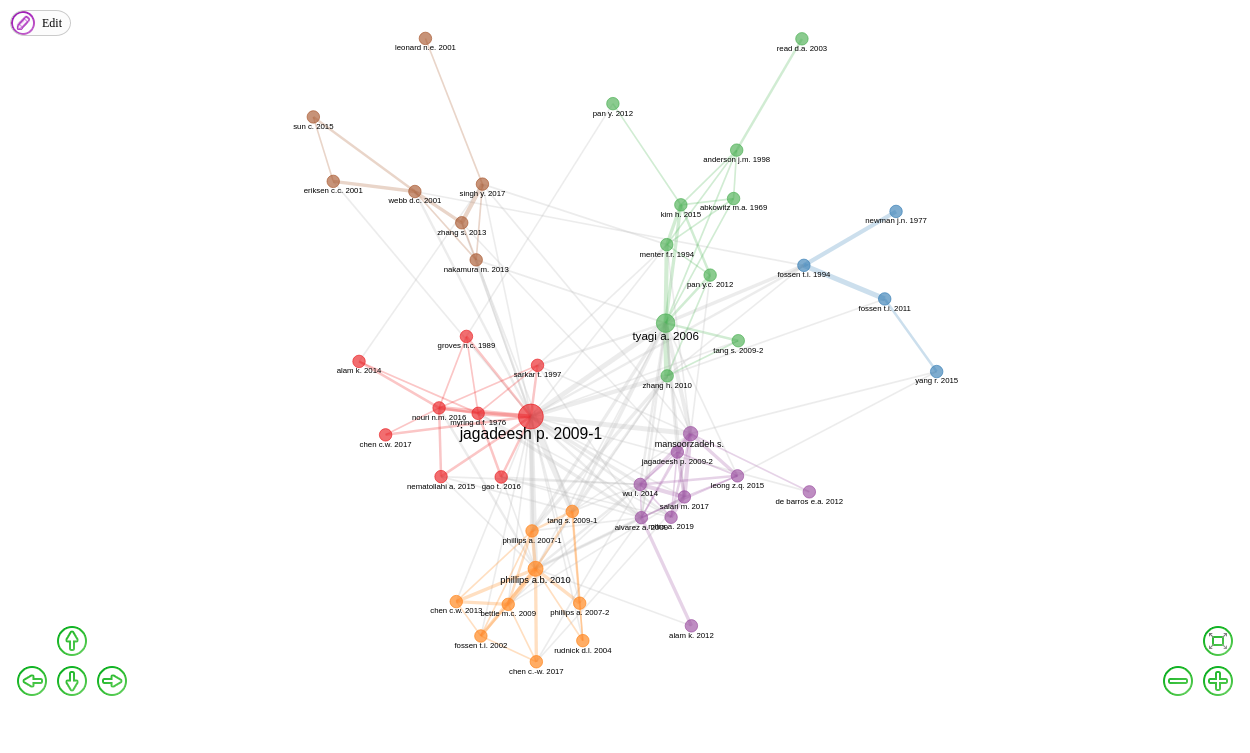
\includegraphics[width=1\textwidth, trim= 200 0 200 0, clip]{turbot4.png}

    \end{columns}

%*----------- notes
    \note[item]{Notes can help you to remember important information. Turn on the notes option.}
\end{frame}
%-
%*----------- SLIDE -------------------------------------------------------------
\begin{frame}[c]{Ciclo Otimizado}
    
    \begin{columns}
        \column{.01\textwidth}
        \column{.5\textwidth}
            \centering
            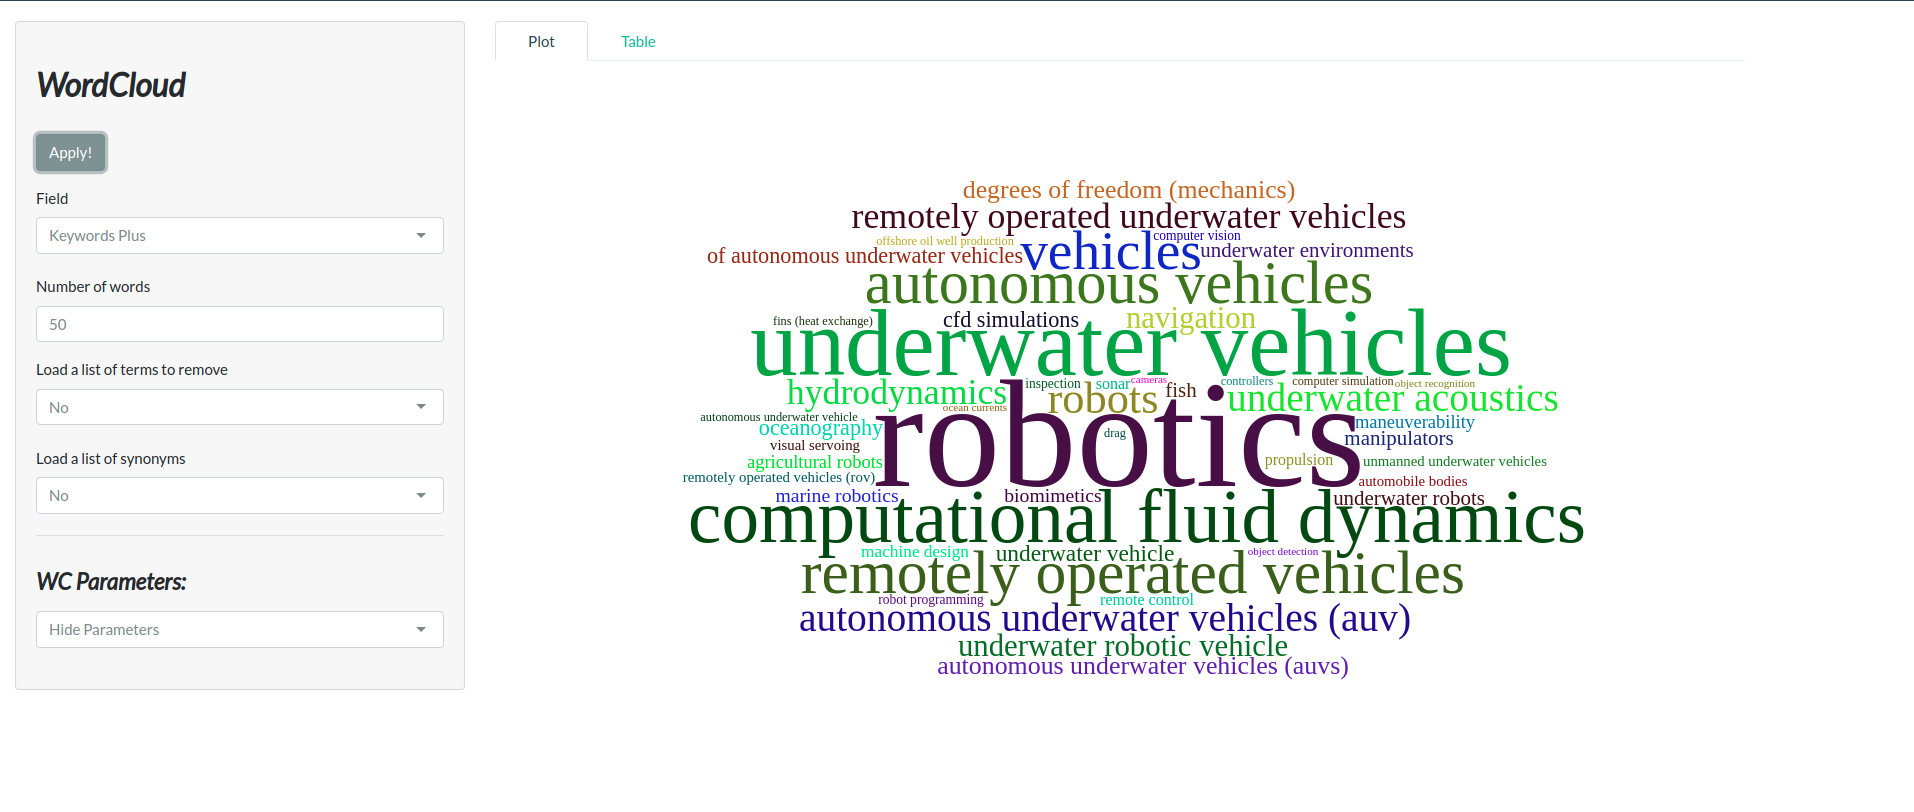
\includegraphics[width=1\textwidth, trim= 600 0 200 0, clip]{turbot5.png}
        \column{.5\textwidth}
            \centering
            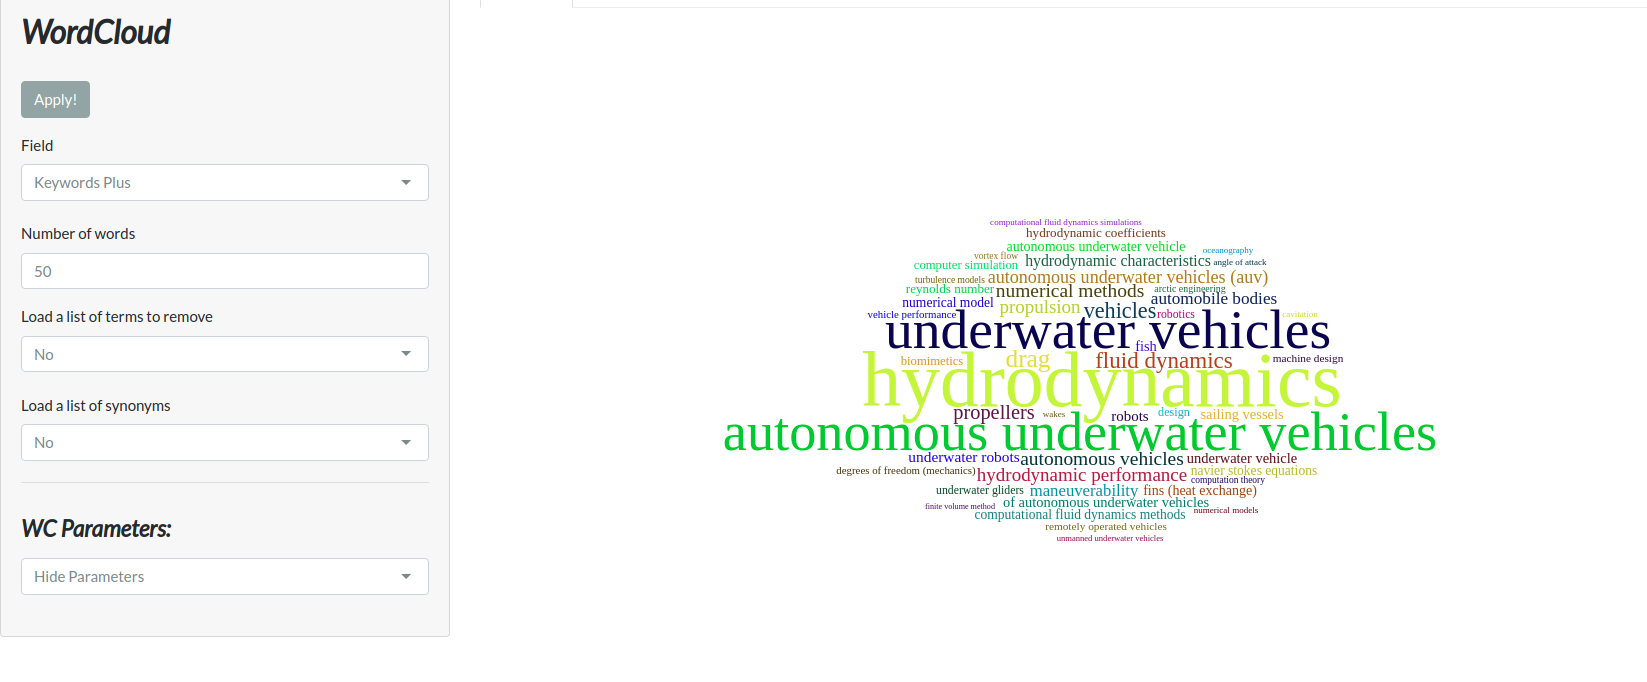
\includegraphics[width=1\textwidth, trim= 700 50 200 100, clip]{turbot6.png}

    \end{columns}

%*----------- notes
    \note[item]{Notes can help you to remember important information. Turn on the notes option.}
\end{frame}
%-
%*----------- SLIDE -------------------------------------------------------------
\begin{frame}[c]{Ciclo Otimizado}
    \framesubtitle{aplicando o RevTools}
    \begin{columns}
        \column{.01\textwidth}
        \column{.5\textwidth}
            \centering
            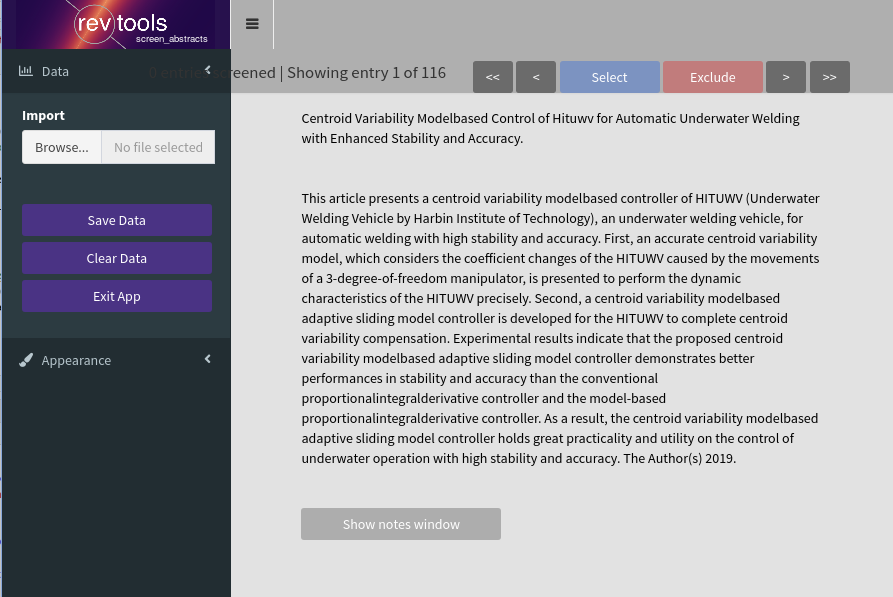
\includegraphics[width=.95\textwidth, trim= 0 0 0 0, clip]{revtools.png}
        \column{.5\textwidth}
    
            O \emph{RevTools} é um pacote do R utilizado para apoiar os pesquisadores que trabalham em projetos de síntese de evidências. \\
            Propicia a visualização baseada em padrões bibliográficos.\\
            Neste método, ele irá promover a exclusão dos artigos que não tem referência com o devido estudo.

    \end{columns}

%*----------- notes
    \note[item]{Notes can help you to remember important information. Turn on the notes option.}
\end{frame}
%-
%*----------- SLIDE -------------------------------------------------------------
\begin{frame}[c]{Ciclo Impacto}
    \begin{columns}
        \column{.01\textwidth}
        \column{.5\textwidth}
            \centering
            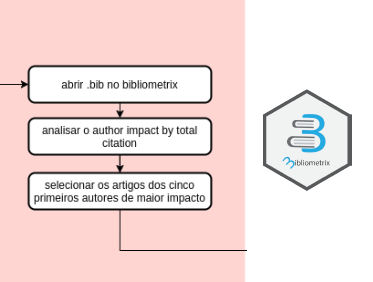
\includegraphics[width=.95\textwidth, trim= 0 0 0 0, clip]{ciclo3.png}
        \column{.5\textwidth}
            Alguns pontos importantes nesta fase:
            \begin{itemize}
                \item Analisar o impacto do autor.
                \item Analisar o impacto do autor por total de citações.
                \item Selecionar os artigos principais dos cinco mais impactantes autores.
            \end{itemize}
        
    \end{columns}

%*----------- notes
    \note[item]{Notes can help you to remember important information. Turn on the notes option.}
\end{frame}
%-
%*----------- SLIDE -------------------------------------------------------------
\begin{frame}[c]{Ciclo Impacto - indexador H}

    \centering
    \centerline{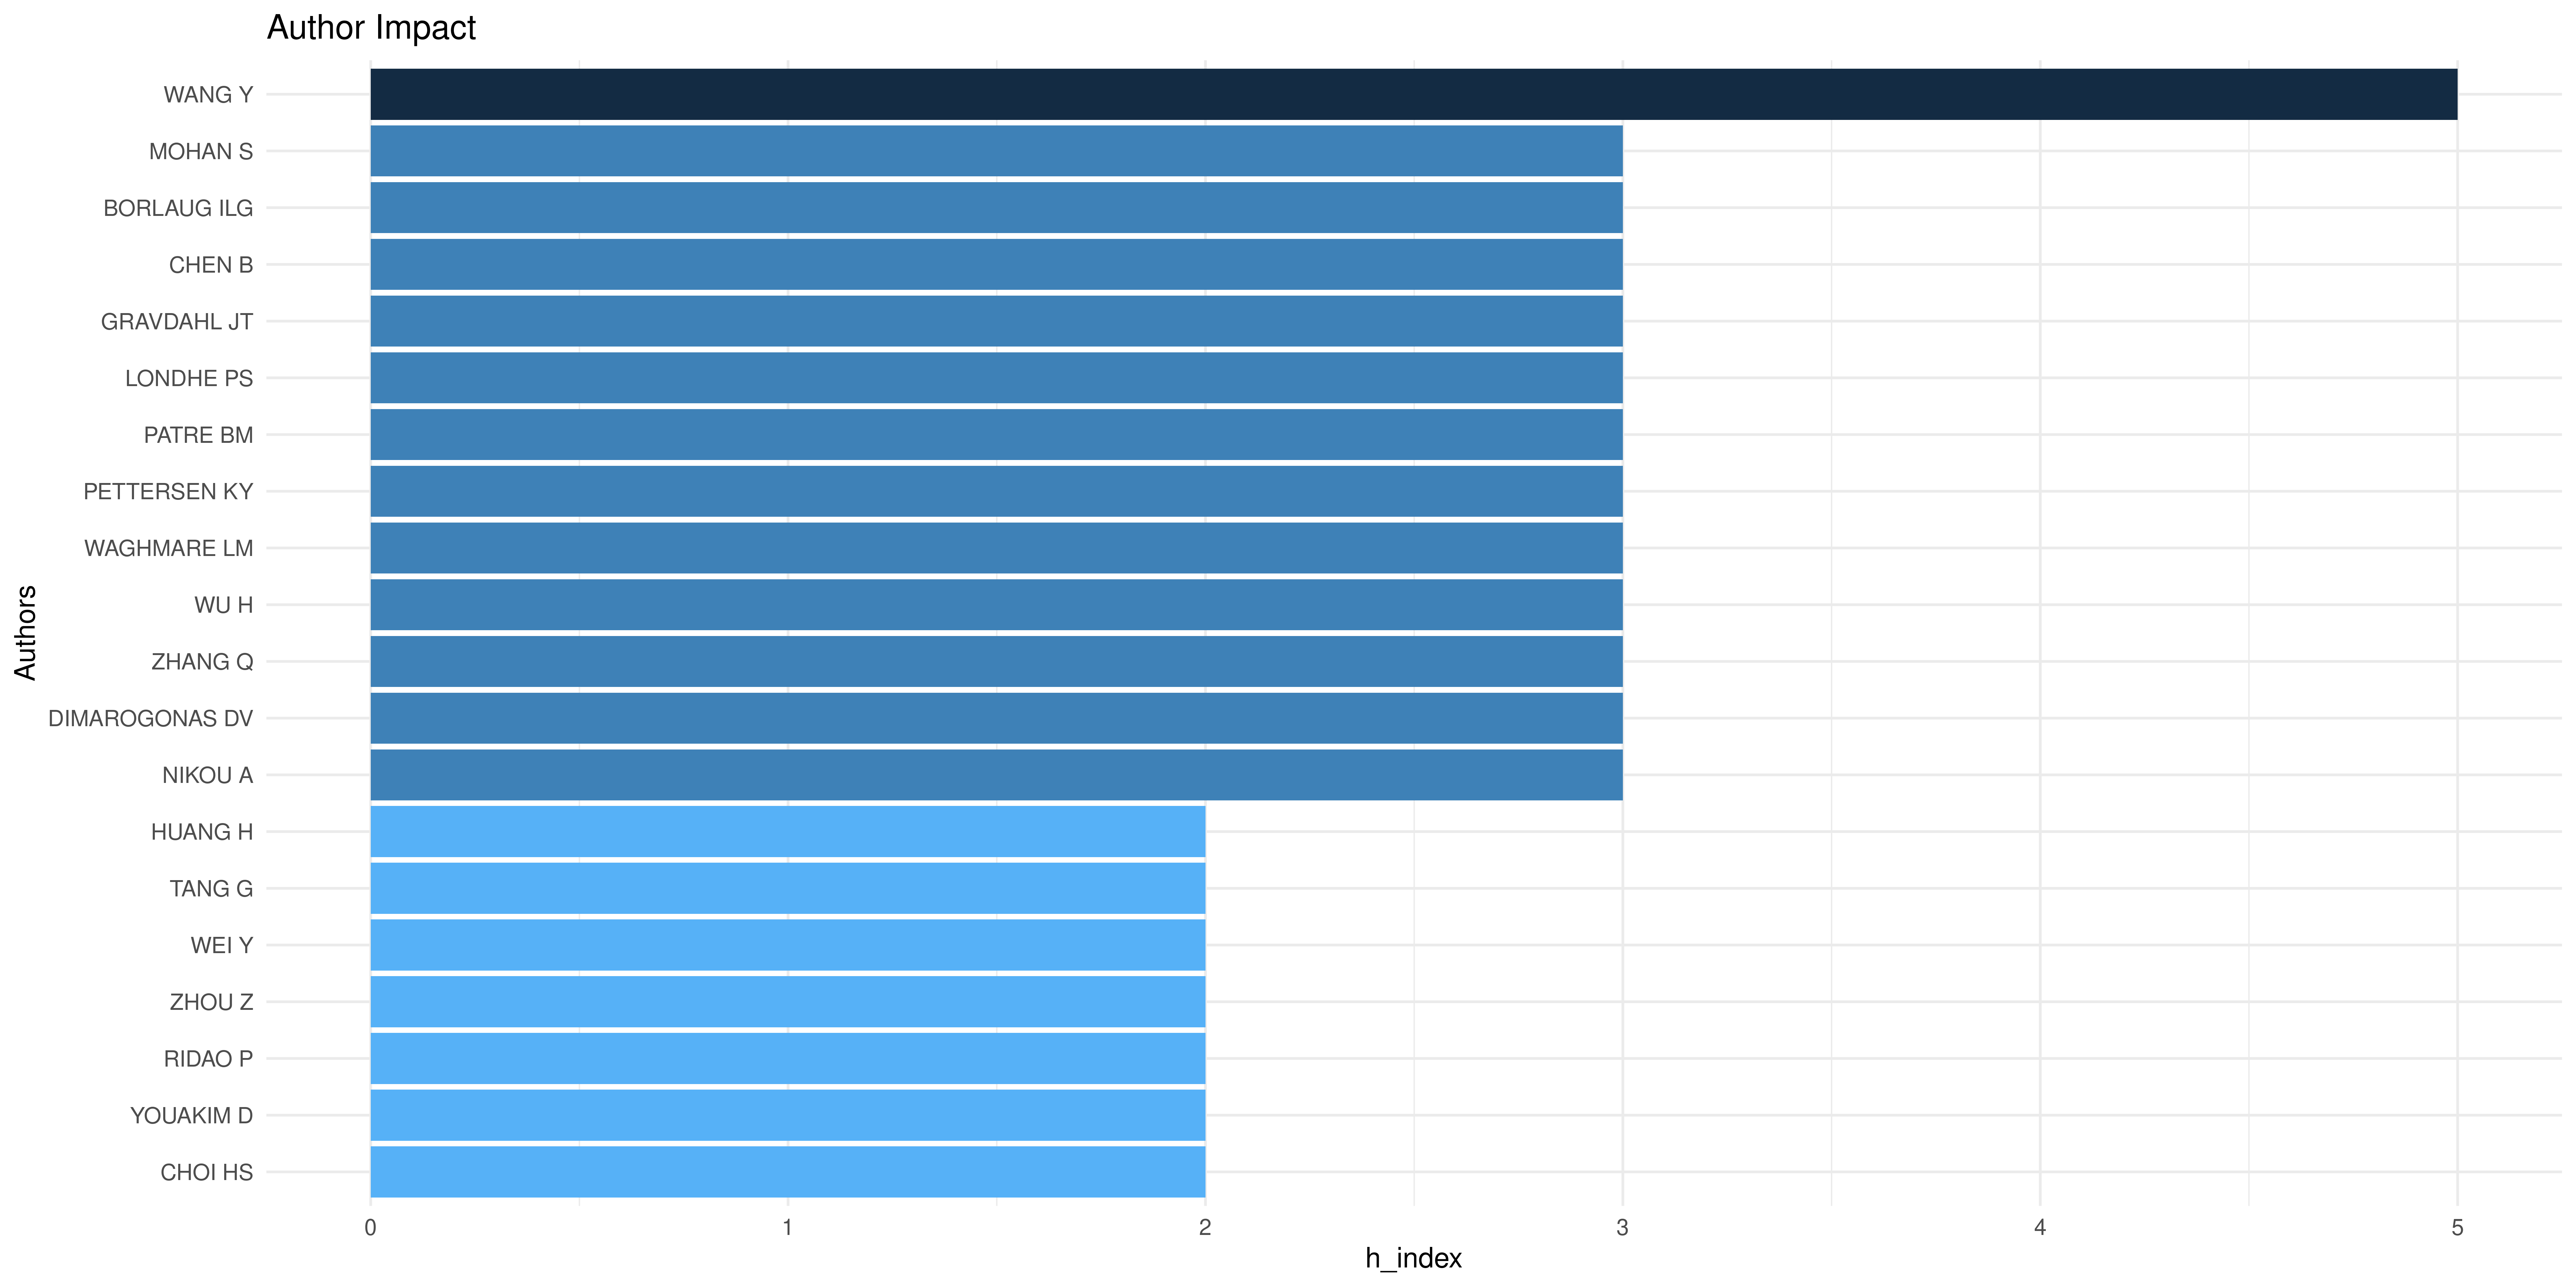
\includegraphics[trim = 0 0 0 0, clip, width=1\textwidth]{AuthorImpact-2021-04-28.png}}

%*----------- notes
    \note[item]{Notes can help you to remember important information. Turn on the notes option.}
\end{frame}
%-
%*----------- SLIDE -------------------------------------------------------------
\begin{frame}[c]{Ciclo Impacto}

    \centering
    \centerline{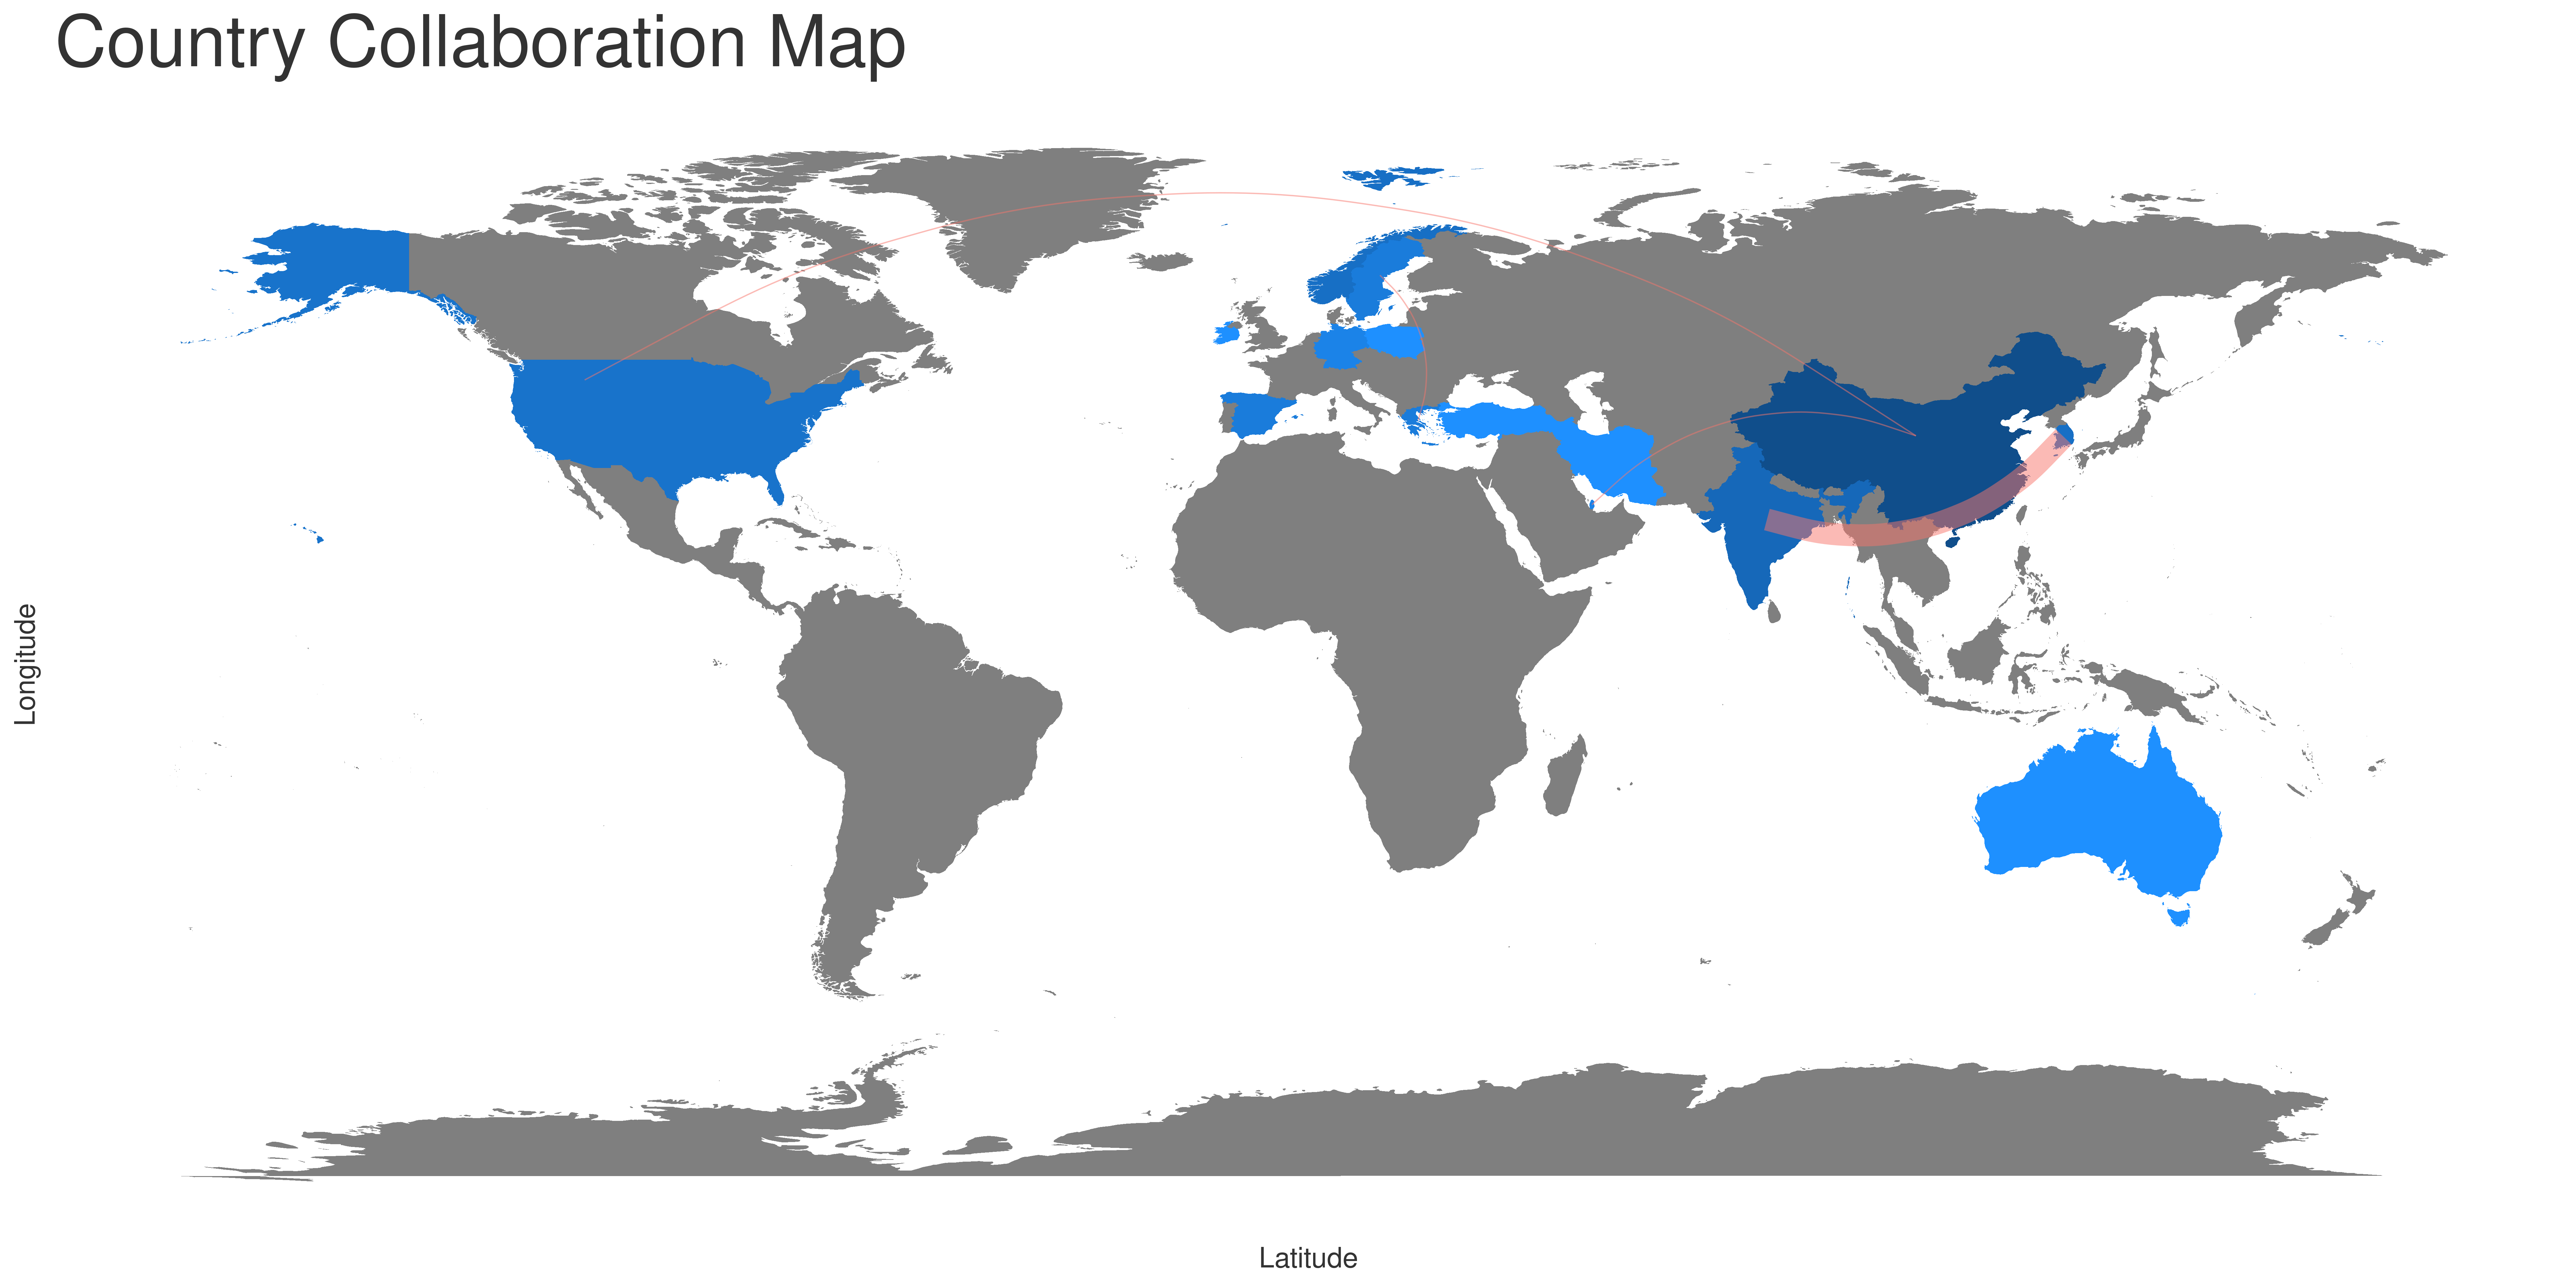
\includegraphics[trim = 0 0 0 40, clip, width=1\textwidth]{CountryCollaborationMap-2021-04-28.png}}

%*----------- notes
    \note[item]{Notes can help you to remember important information. Turn on the notes option.}
\end{frame}
%-
%*----------- SLIDE -------------------------------------------------------------
\begin{frame}[c]{Ciclo Produção}
    \begin{columns}
        \column{.01\textwidth}
        \column{.5\textwidth}
            \centering
            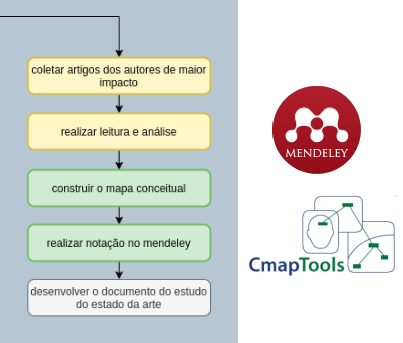
\includegraphics[width=.95\textwidth, trim= 0 0 0 0, clip]{ciclo4.png}
        \column{.5\textwidth}
            Gerar documentos de análise.

            \centering
            \begin{figure}
                     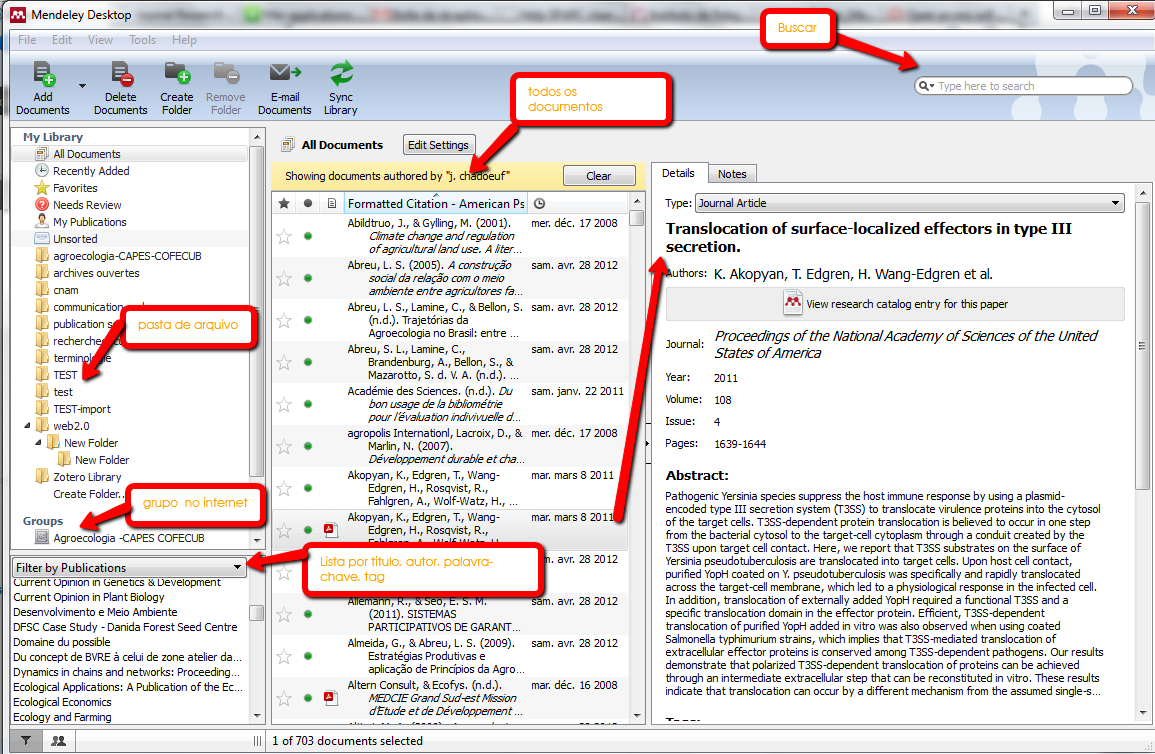
\includegraphics[width=0.7\textwidth]{mendeley.png}
                     \hfill
                     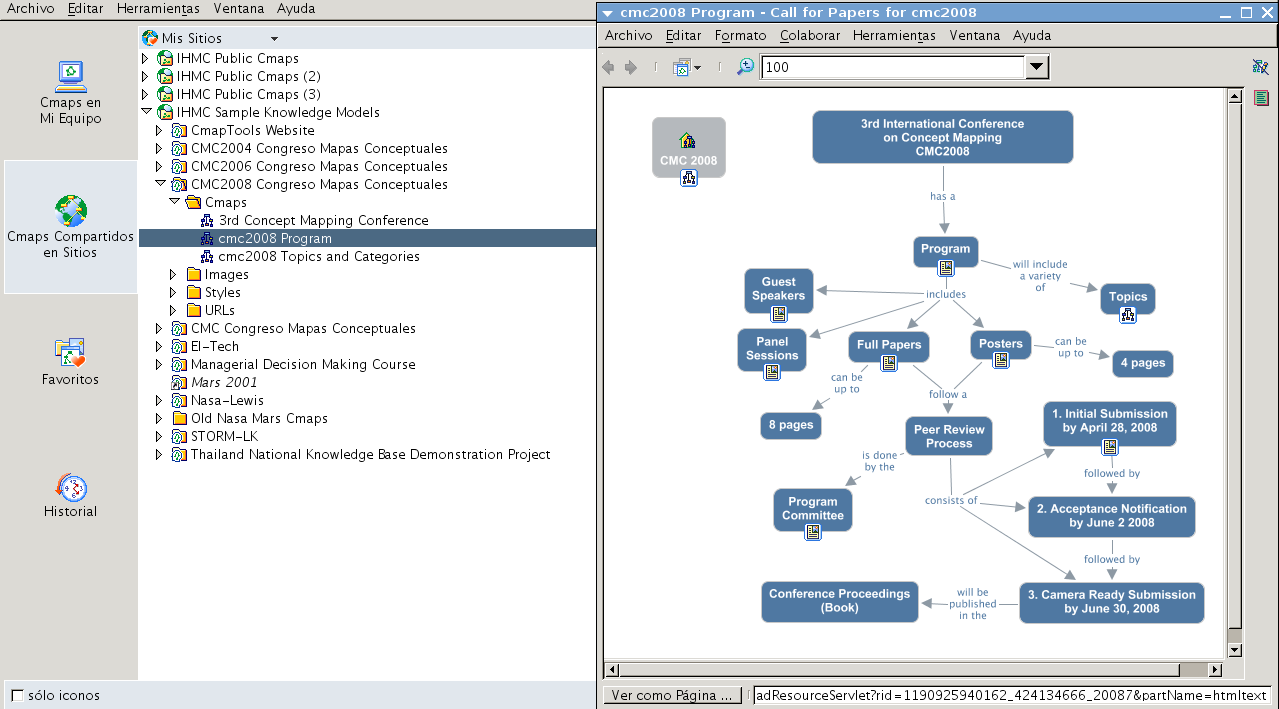
\includegraphics[width=0.7\textwidth]{cmaptools.png}
            \end{figure}
        
    \end{columns}

%*----------- notes
    \note[item]{Notes can help you to remember important information. Turn on the notes option.}
\end{frame}
%-
%*----------- SLIDE -------------------------------------------------------------
\begin{frame}[c]{Ciclo Produção}
    \centering
    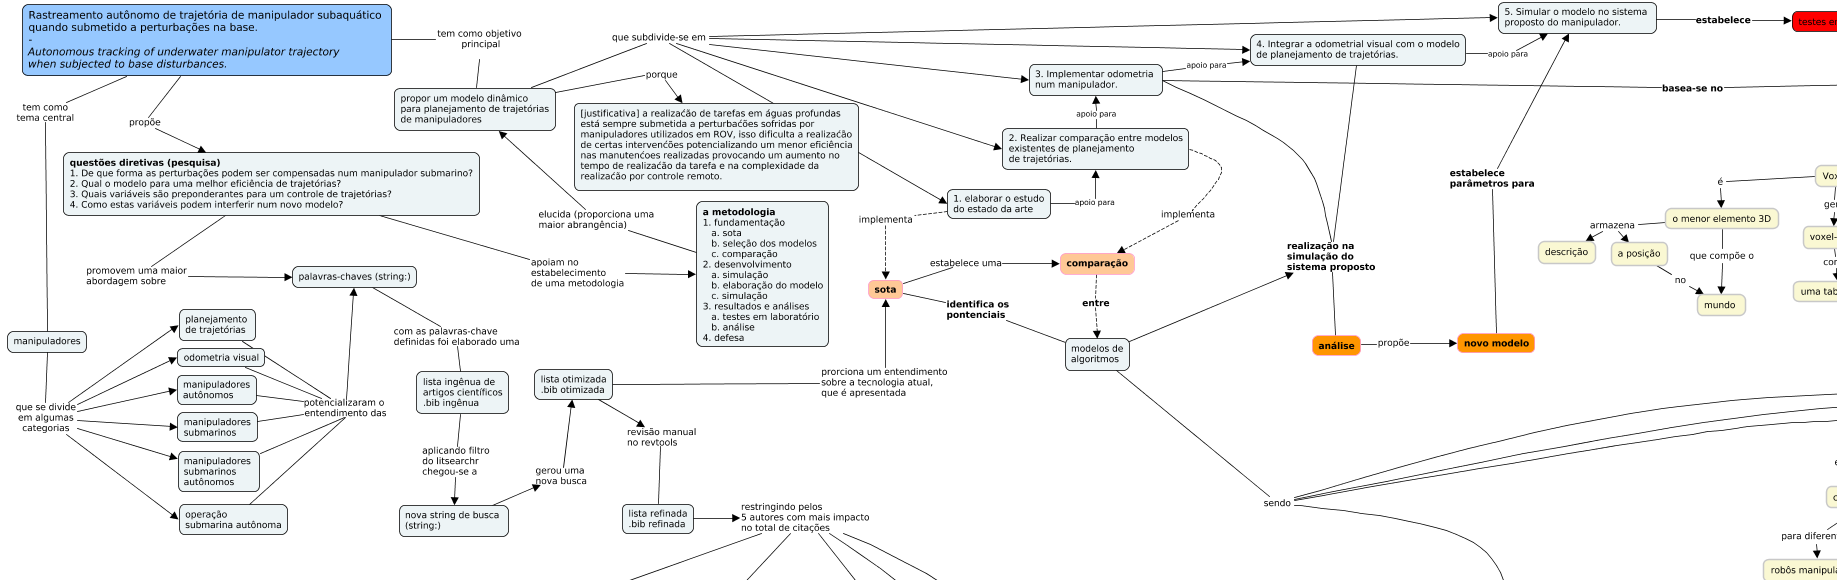
\includegraphics[width=1.5\textwidth, trim = 0 0 300 0, clip]{mapa-conceitual-recorte.png}

%*----------- notes
    \note[item]{Notes can help you to remember important information. Turn on the notes option.}
\end{frame}
%-
%*----------- SLIDE -------------------------------------------------------------
{
\setbeamertemplate{background}
{
\includegraphics[width =\the\paperwidth, clip, trim = 0 0 0 100]{nick-morrison-FHnnjk1Yj7Y-unsplash.jpg}}
%*----------- SLIDE -------------------------------------------------------------
\begin{frame}[t]{} 
\end{frame}
}
%-
%*----------- SLIDE -------------------------------------------------------------
\begin{frame}[c]{}
    \centering
    
\includegraphics[width=.65\textwidth, trim= 0 0 0 0, clip]{github.png}
    
    \vspace*{0.3cm}
    \href{https://github.com/Brazilian-Institute-of-Robotics/bir-mini-method-bili}{link-do-repositório}
%*----------- notes
    \note[item]{Notes can help you to remember important information. Turn on the notes option.}
\end{frame}
%-